\chapter{The Database}
In this chapter the database design and implementation is presented.  
\section{Design}
In the parent control system there are seven essential objects; control system, profiles, tags, controller, chores, rules and permission. 


\begin{description}
	\item[Control system] is identifying the individual system and all of the other objects are connected to a control system.
	\item[Profile] is a representation of a specific person in the control system. The person can both be a child or the parent, but this should be distinguishable.
	\item[Tag] identifies the physical tag that a profile uses to activate the controllers. A tag is identified by the serial number of the physical tag.
	\item[Controller]	is a object representation of the physical controller and like the tag it is identified by the serial number of the physical controller.
	\item[Chore] is a representation of a house chore which can be carried out by a child (profile) which then gets point as a reward.
	\item[Permission] is representing time restrictions on the controllers which some of the profiles need to abide by. 
	\item[Rule] is representing other restriction or rules that cannot be expressed by the permission. An example could be the Playstation may not be turned on unless the TV has been turned on. A rule consist of some conditions that need to meet before some actions should be taken. 
\end{description}

From the former description the database design is made. The design is represented in a ER schema where the cardinality ratio is expressed in 
Chen notation. The ER schema is shown in figure \ref{fig:ERdiagram}. 

\begin{figure}
	\centering
		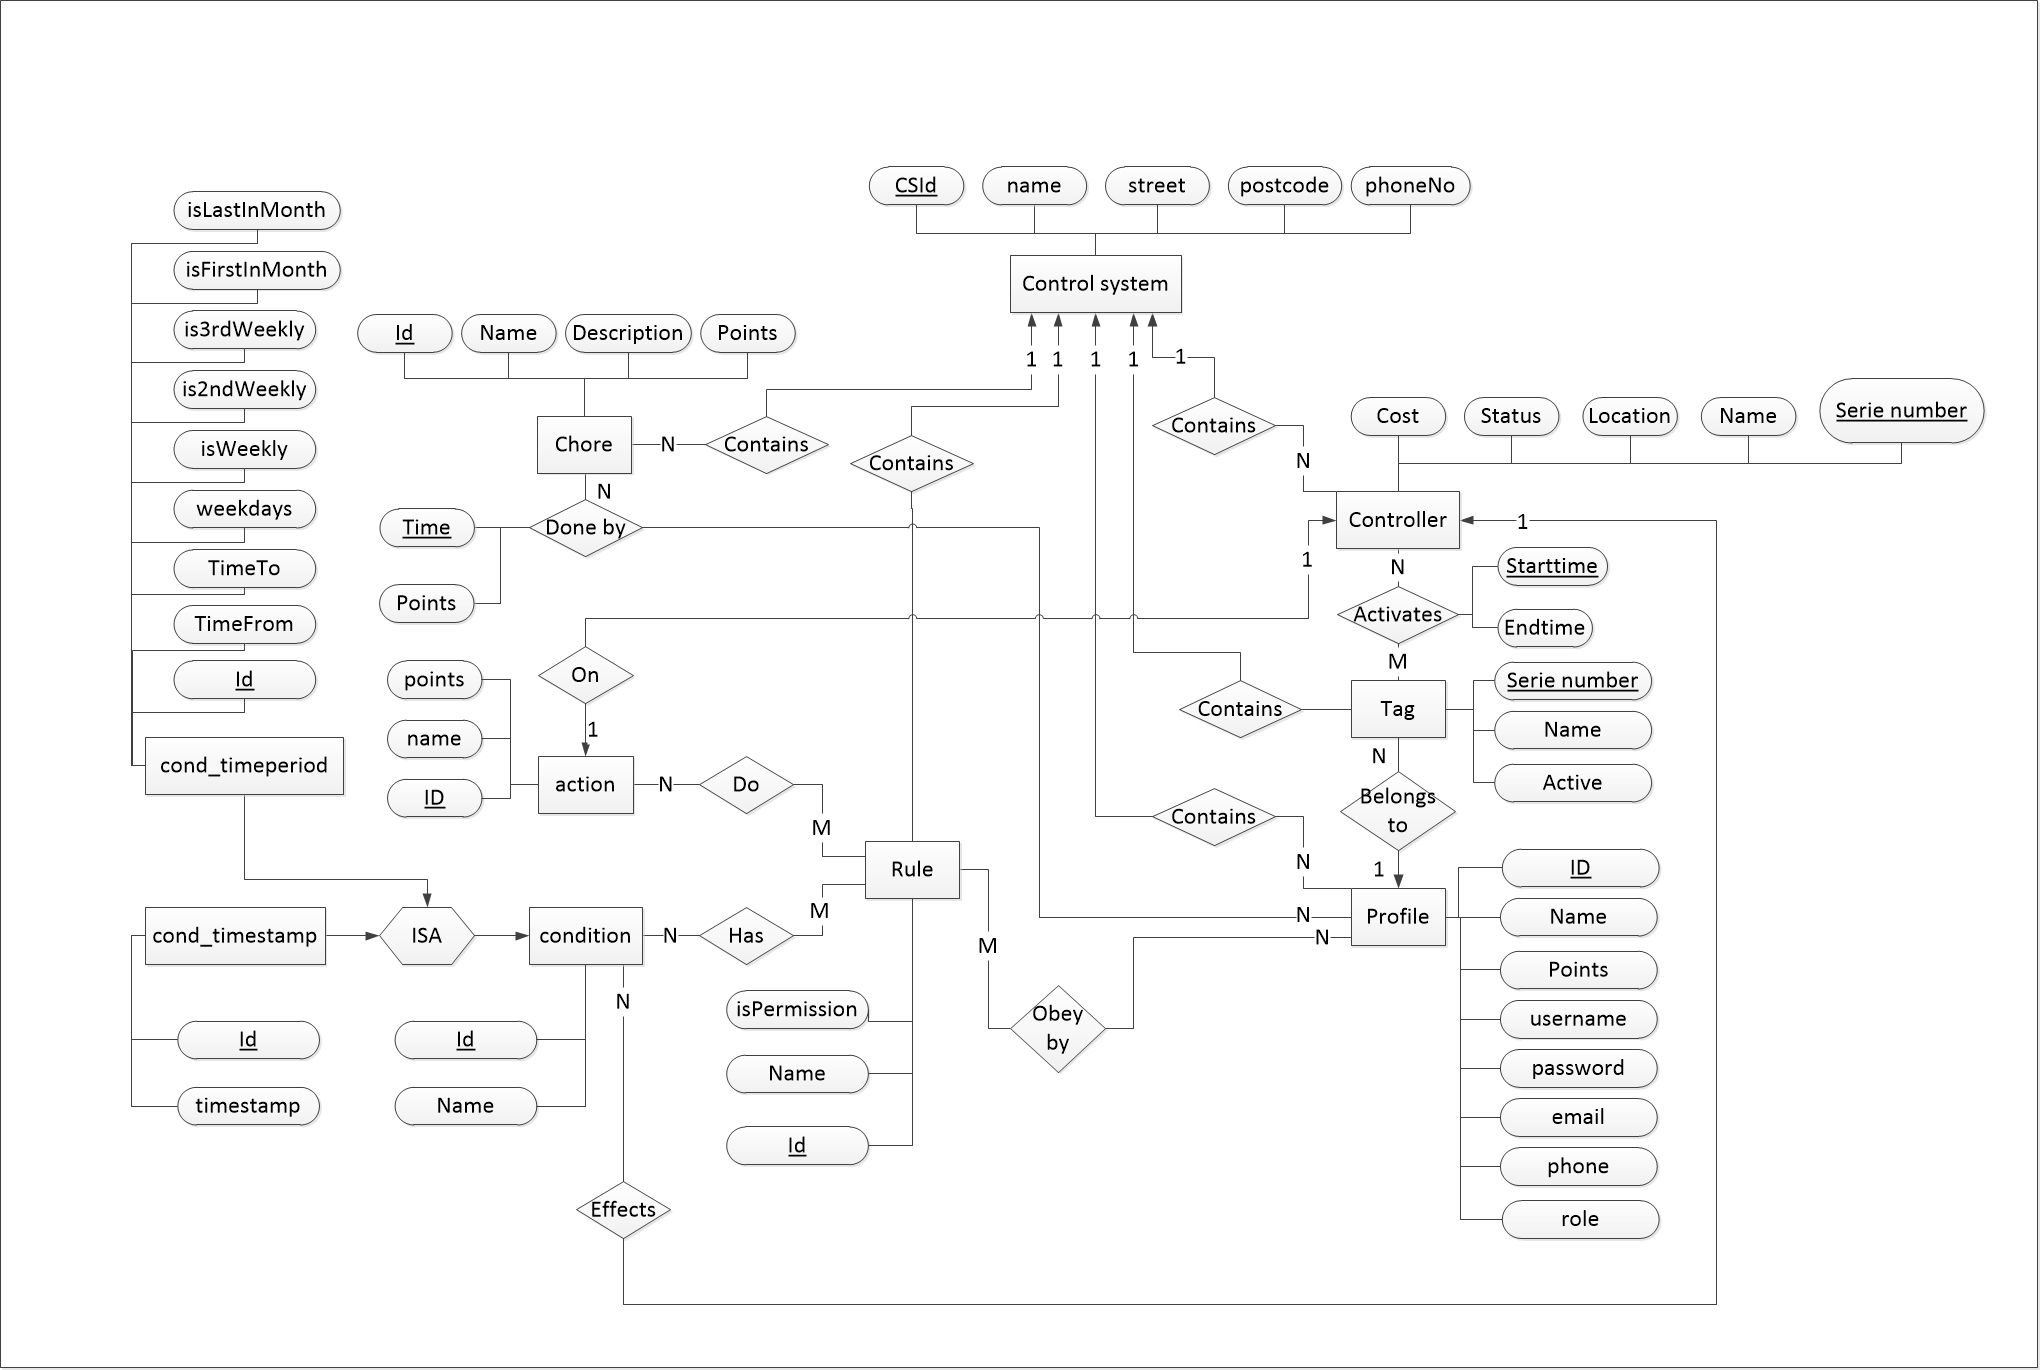
\includegraphics[width=1.00\textwidth]{images/ERdiagram.jpg}
	\caption{ER schema of the database design}
	\label{fig:ERdiagram}
\end{figure}

In the database design it should be noticed that Permission is absent. The reason is that for every permission that could be made a similar rule can be made but not every rule can be represented as a permission. Therefore the data representation of Permission is the same as Rule. However, on the website the two should be represented differently and so the attribute \texttt{isPermission} have been add to Rule which will difference the two.

Another observation in the design is the condition of a rule. The condition can be one of three representations. The first is the simplest because it is just the Condition. The second is Condition and a timestamp which is the \texttt{cond\_timestamp} in the design in \ref{fig:ERdiagram}. The last representation is Condition, a time period, and a representation of when it is valid, which in the design is \texttt{cond\_timeperiod}. Since the \texttt{cond\_timeperiod} is the more advanced of the three it will later be explained further including with some examples. It is the name of the condition which distinguishes with representation should be used. If the name is \texttt{Timestamp} it should be cond\_timestamp, if it is \texttt{Timeperiode} then it is cond\_timeperiod and any other name it is only the Condition.


As can be seen in \texttt{cond\_timeperiod} it has several attributes to represent when the time period is valid, because it is repeatable. An example could be that the profile Peter gets point for each football training and the football training is Monday and Thursday from 18:00 to 19:30 each week. Another example could be that the family are going out every third Saturday at 18:00 and to get the children away from the media devices in time then the TV,PC and consoles must not be turn on from 17:30 to 18:00. 

After the design in the ER-schema was completed it was implemented into a MySQL database.  

\section{Implementation}

The design from figure \ref{fig:ERdiagram} has been implemented in a MySQL database and the result can be found in figure \ref{fig:databaseDiagram}. The schema is in 3NF
%sql or diagram
\begin{figure}
	\centering
		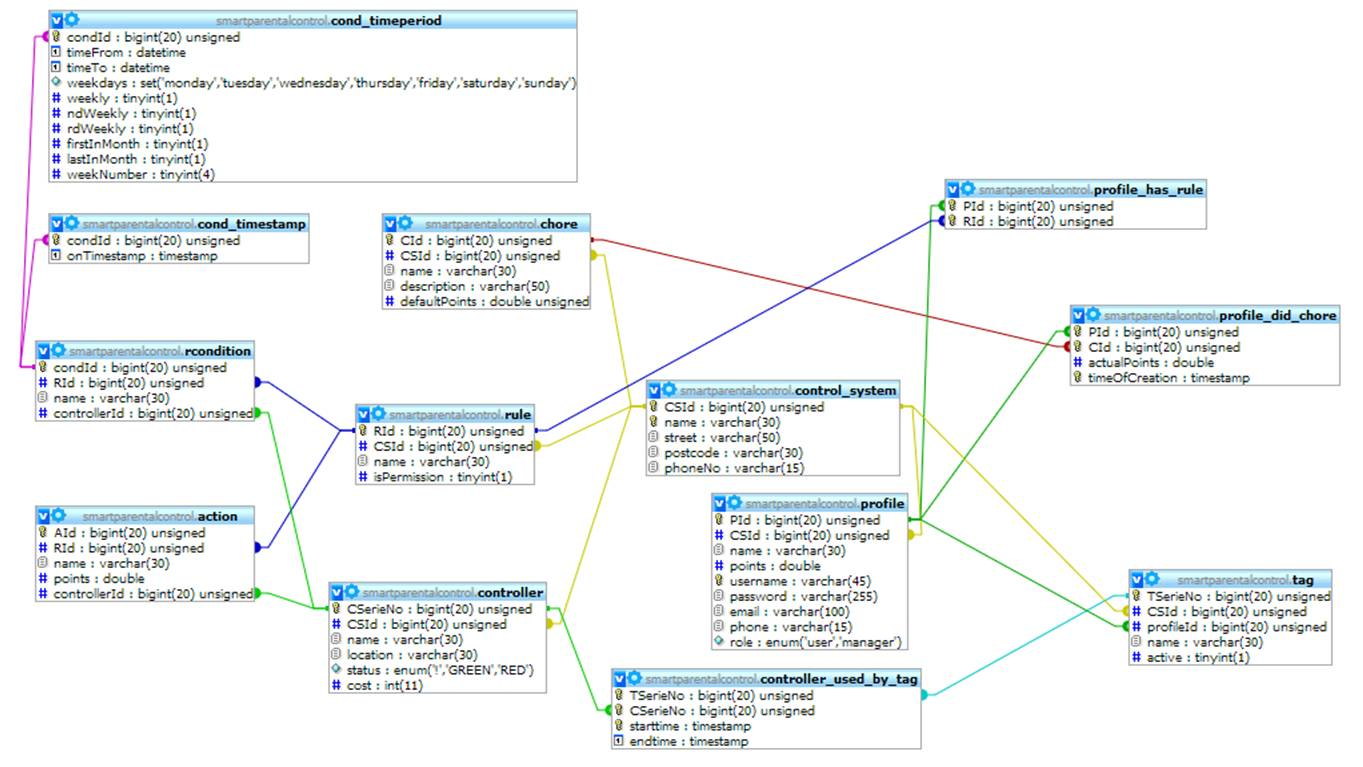
\includegraphics[width=1.00\textwidth]{images/databaseDiagram.jpg}
	\caption{The Database implementation}
	\label{fig:databaseDiagram}
\end{figure}

%delete cascade




%sql Helper class
\subsection{sql Helper class}